\section{Summary and future work} 
\label{summary}

We measured the performance of both the sequential and the auto-parallel versions of SPEC2000FP benchmarks. The results are shown in Figure~\ref{fig:performance}\footnote{The numbers shown here are based
  on a snap shot of our development compiler.}.The figure shows three execution times for each benchmark,
\begin{itemize}
\item \emph{Sequential} : sequential execution time of the benchmark code compiled by our compiler at the highest
optimization level.
\item \emph{Parallel} : parallel (2 threads) execution time of the benchmark parallelized by the auto-parallelizer for SMP machines.
\item \emph{Improved} : parallel (2 threads) execution time with manual changes to the source code as described in Section \ref{opportunities}
\end{itemize}

\begin{figure}[h!]
  \begin{center}
    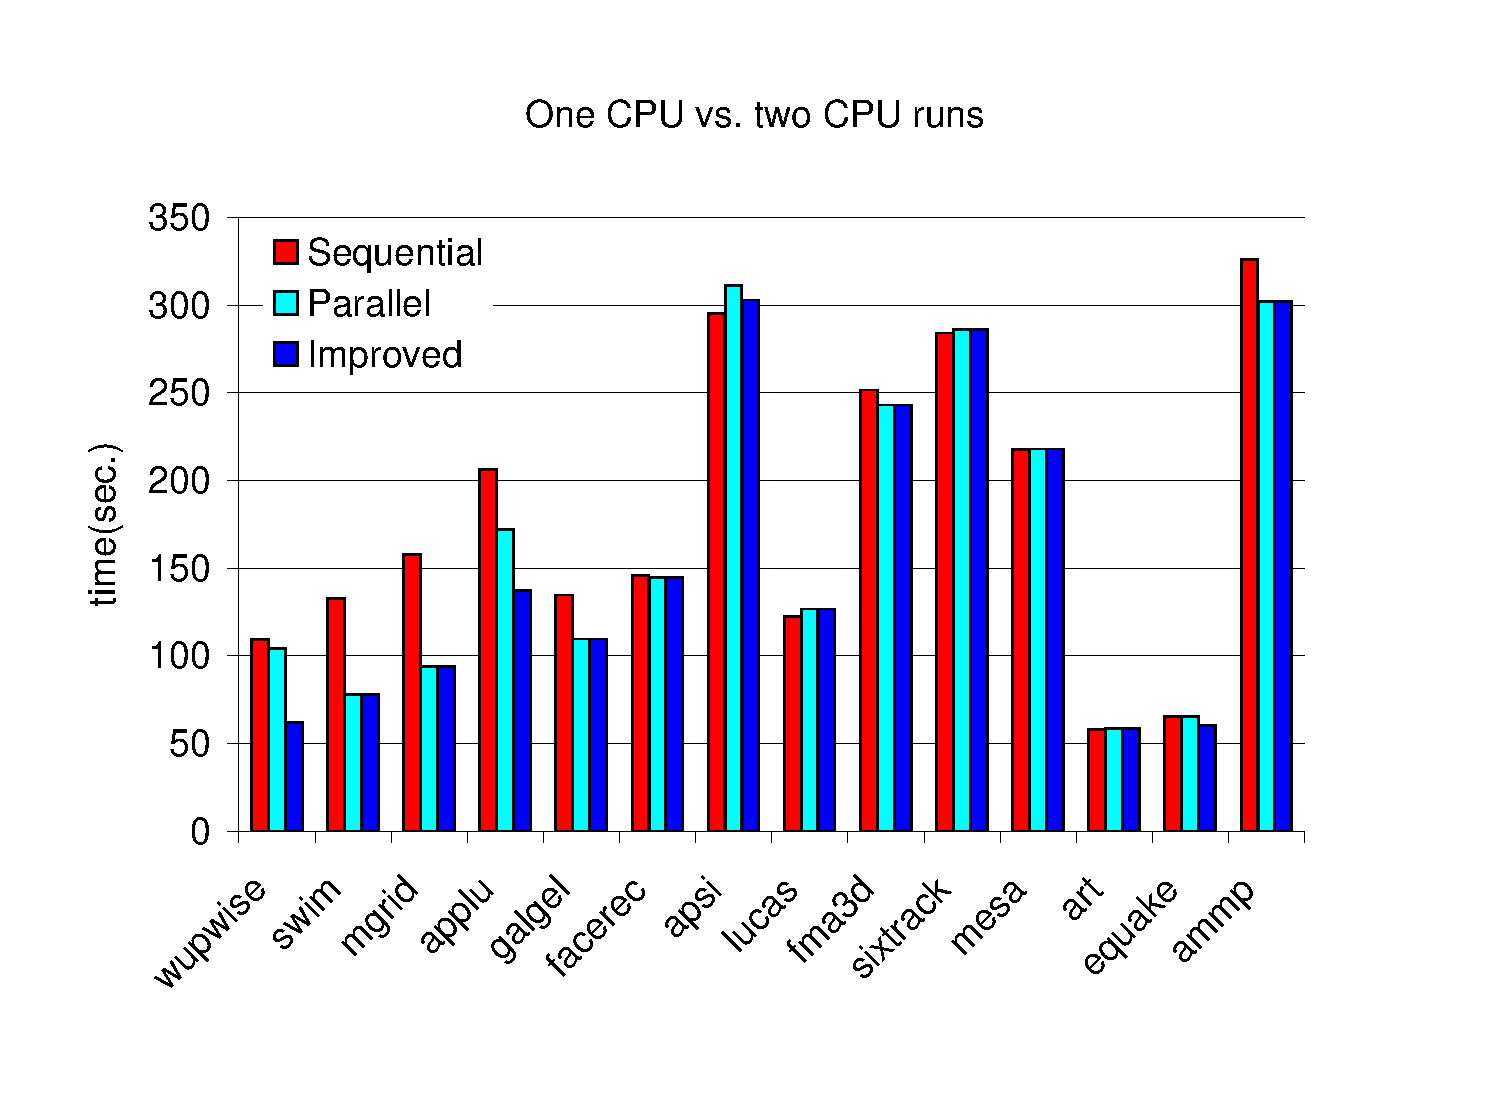
\includegraphics[angle=0, width=0.85\textwidth]{spec2kfp.eps}
    \caption{\footnotesize Performance of auto-parallelization}
    \label{fig:performance}
  \end{center}
\end{figure}

We also emphasize that for simplicity, the modification to individual benchmarks for the \emph{Improved} results address only one specific problem among the 3 identified in Section \ref{opportunities}. For instance, \texttt{apsi} 
is affected by zero trip loops, function calls in the loop body as well as array privatization. However, the source modification includes only source changes for zero trip loops. Among those 10 benchmarks in the SPECOMP test suite, \texttt{swim}, \texttt{mgrid}, \texttt{applu}, \texttt{galgel} and \texttt{wupwise}
see reasonable speedup, with improvement up to 40\%.

The results from auto-parallelization as shown by Figure ~\ref{fig:performance} are not very impressive, especially considering that the hardware resource has actually doubled. However, we argue that the focus in this paper has been the utilization of simple techniques to achieve parallelization with minimal impact on the compilation time. This paper has also shown that much better performance is obtainable using sophisticated techniques at the cost of increased compilation time. In addition, this paper also presents a simple loop permutation algorithm to balance data
locality and coarse-grained parallelism on SMP machines.


Our auto-parallelizer has several limitations as shown in Section \ref{opportunities}. Implementing array privatization analysis and improving the existing dependence analysis are part of the planned future work. We also plan to fine-tune several heuristics and guidelines used in the parallelizer. With all these improvements, we hope that the auto-parallelizer will be able to detect inherent parallelism in the application code on par with explicit parallelization if not better.

